\documentclass[conference]{IEEEtran}
\IEEEoverridecommandlockouts
% The preceding line is only needed to identify funding in the first footnote. If that is unneeded, please comment it out.
\usepackage{cite}
\usepackage{amsmath,amssymb,amsfonts}
\usepackage{algorithmic}
\usepackage{graphicx}
\usepackage{textcomp}
\usepackage{xcolor}
\def\BibTeX{{\rm B\kern-.05em{\sc i\kern-.025em b}\kern-.08em
    T\kern-.1667em\lower.7ex\hbox{E}\kern-.125emX}}
\begin{document}

\title{Principal Component Analysis (PCA) for dimension reduction.\\

}

\author{\IEEEauthorblockN{1\textsuperscript{st} Coder\_225}
\IEEEauthorblockA{\textit{dept. Computer Science} \\
13228201005@163.com}
}

\maketitle

\begin{abstract}
In recent years, the collection of huge and diverse data has opened challenges to data analysis. Most of these data contain an important amount of redundant data. The researchers aim to feed the data into the model that will then generalize patterns within the data and utilize the data in a sophisticated way to solve a variety of real-world problems. To efficiently extract valuable insight from multidimensional data with a huge number of variables, it is essential to reduce the number of variables and interpret the linear combination of the data. Principal Component Analysis (PCA), is a dimensionality-reduction method, that uses sophisticated mathematical principles to reduce the dimensionality of a large dataset, meaning reducing the number of features while maintaining the necessary information present in the original dataset. This research aims to provide a complete understanding of the PCA approach to dimensionality reduction. The paper shows the representation and visualization of the Iris dataset after applying PCA which results in the use of a smaller number of variables for the representation.
\end{abstract}

\begin{IEEEkeywords}
PCA, Iris dataset, dimension reduction
\end{IEEEkeywords}

\section{Introduction}
Data visualization represents an important step in understanding and analyzing voluminous data~\cite{Lamrini}, given n-dimensional data, the representation of the data is not always as straightforward as it may seem. One-dimensional data is a simple representation of the data on the number line. Also, the two-dimensional data is represented by xy-plane, and three-dimensional data is the space. In recent years, there has been an increase of data in various fields, the amount of multidimensional data created is increasing at an exponential rate, it is predicted to reach 44 zettabytes in 2020~\cite{Genender}. Although, for data with a dimension higher than three, representation and visualization become more complex. Moreover, the data need to be analyzed and valuable features need to be extracted therefore, obtaining significant information from the dataset becomes difficult due to high dimensionality and number of variables. In this context, to tackle these challenges, numerous data reduction methods have been developed over the last decades~\cite{Liu} nonetheless, the need for new visualization approaches remains~\cite{Onana}. The dimensionality reduction represents an originally high dimension data in a new form with a smaller dimensional space value with the inevitable loss of information. In practice, the high dimensional data must be converted one way or the other into a low dimensional geometry for display~\cite{Xu}. Also, traditional approach such as bivariate plots tends to find the relationship between variables however, the feasibility of this method becomes impractical for a large dataset as it requires $n!/2!(n-2)!$ plots.
PCA is a method of mathematical transformation that aims to classify major variables that account for variances in the given data called principal components. The detection of these variables leads to a more compressed explanation of data associations and thus to a clearer understanding of the underlying characteristics. Therefore, in a dataset, it is an effective approach to derive general patterns. Besides, since PCA offers principal components ordered by their significance, it represents an excellent basis for the reduction of the data dimension in the case of multidimensional data~\cite{Nocke}. PCA uses a transformation of vector space to decrease the dimensionality of huge datasets. In high-dimensional data, it seeks the highest variance directions that is equal to the least square line of best fit through the plotted data and projects it to a smaller dimensional subspace while maintaining most of the data. The PCA method describes the contributions of each principal component, the total variance, and the eigenvectors associated with non-zero eigenvalues~\cite{Salem}. 
The remainder of this paper is organized as follows: Section II is dedicated to the related work that falls within the scope of our research. In section III, the fundamental of PCA is introduced. We propose our PCA algorithm with the implementation steps in section IV. We implement and discuss the result in Section V and we conclude this paper in Section VI.


\section{Related work}

Dimensionality reduction has gained a lot of attention in recent years. Great efforts have been expended to provide solutions methods, amongst which we can cite the work in~\cite{Houari}, the author proposed Copulas and LU-decomposition technique for dimensionality reduction, the algorithm was tested and showed satisfying result on real-world datasets such as Diabetes, Waveforms, Human Activity Recognition based on Smartphone and Thyroid Datasets. In~\cite{Menon}, the algorithm proposed by the author performs better than Gaussian-based FSVD for dimensionality reduction in hyperspectral classification. Additionally, in~\cite{Rehman} a detailed discussion of large data reduction methods, including large data compression, dimension reduction, redundancy elimination, data mining, and machine-theory-based automatic learning methods.~\cite{A} presents the basic definitions of the PCA technique along with the calculation of the covariance matrix and Singular Value Decomposition. 

\section{Fundamentals of PCA}
The Principal Component Analysis is a widely used data reduction technique, PCA aims to find the directions or so-called the principal components of maximum variance in high-dimensional data and project it onto a smaller dimensional subspace while retaining most of the information. As in~\cite{D}, a dataset, with  rows representing the variables and columns denoting the observations is expressed in a matrix with row vectors.

\begin{equation}
X=\left( \begin{matrix}
   {{x}_{1,1}} & {{x}_{1,2}} & \cdots  & {{x}_{1,n}}  \\
   {{x}_{2,1}} & {{x}_{2,2}} & \cdots  & {{x}_{2,n}}  \\
   \vdots  & \vdots  & \ddots  & \vdots   \\
   {{x}_{m,1}} & {{x}_{m,2}} & \cdots  & {{x}_{m,n}}  \\
\end{matrix} \right)=\left( \begin{matrix}
   {{X}_{1}}  \\
   {{X}_{2}}  \\
   \vdots   \\
   {{X}_{m}}  \\
\end{matrix} \right)\
\end{equation}

The linear transformation of the matrix $X$ into ${{Y}_{m\times n}}$ by using a ${{P}_{m\times m}}$ matrix with row vectors ${{p}_{1}},{{p}_{2}},...,{{p}_{m}}$ and column vectors of the matrix  denoting by ${{x}_{1}},{{x}_{2}},...,{{x}_{n}}$,

\begin{equation}
{{Y}_{m\times n}}={{P}_{m\times m}}X=\left( \begin{matrix}
   {{p}_{1}}\cdot {{x}_{1}} & {{p}_{2}}\cdot {{x}_{2}} & \cdots  & {{p}_{3}}\cdot {{x}_{n}}  \\
   {{p}_{2}}\cdot {{x}_{1}} & {{p}_{2}}\cdot {{x}_{2}} & \cdots  & {{p}_{2}}\cdot {{x}_{n}}  \\
   \cdots  & \cdots  & \ddots  & \cdots   \\
   {{p}_{m}}\cdot {{x}_{1}} & {{p}_{m}}\cdot {{x}_{2}} & \ldots  & {{p}_{m}}{{x}_{n}}  \\
\end{matrix} \right)
\end{equation}

The dot product ${{p}_{i}}\cdot {{x}_{j}}$ is the projection of the original dataset $X$ on the columns of the matrix $P$. Here, the new basis represented by the rows of denotes the principal component directions. In the following part, we introduce the steps required for PCA analysis.

\subsection{Standardize the variables}
This denotes the very first step of PCA, we perform standardization to rescale the features in a way that they have the properties of a standard normal distribution with a mean of zero. Indeed, it provides a suitable normalization with equals weights. To do so, the mean value is subtracted from the dataset $S$.
\begin{equation}
{{X}_{i,j}}={{S}_{i,j}}-{{\overline{X}}_{j}}
\end{equation}

\subsection{Covariance matrix}
The covariance matrix includes all covariance pairs between  variables and along the diagonals all variances, as the covariance measures the correlation between variables. the covariance of the standardized matrix is represented as 
\begin{equation}
{{C}_{x}}=\frac{1}{n-1}X{{X}^{T}}=\frac{1}{n-1}\left( \begin{matrix}
   {{x}_{1}}x_{1}^{T} & {{x}_{1}}x_{2}^{T} & \cdots  & {{x}_{1}}x_{m}^{T}  \\
   {{x}_{2}}x_{1}^{T} & {{x}_{2}}x_{2}^{T} & \cdots  & {{x}_{2}}x_{m}^{T}  \\
   \vdots  & \vdots  & \ddots  & \vdots   \\
   {{x}_{m}}x_{1}^{T} & {{x}_{m}}x_{1}^{T} & \cdots  & {{x}_{m}}x_{m}^{T}  \\
\end{matrix} \right)\
\end{equation}
An interpretation of the value of the variance could be expressed as follow, the larger the variance, the more movements and interesting features it represents while the smaller the value, it may be representing noise or unwanted data in the system. Thus, the covariance of ${{C}_{y}}$, the transformed matrix ${{Y}_{m\times n}}$ should maximize the diagonal entries in other words maximize the signal and minimize the covariance between variables by minimizing the off-diagonal entries. Based on the requirements, we choose the matrix ${{P}_{m\times n}}$ with orthogonal vectors ${{P}_{1}},{{P}_{2}},...,{{P}_{m}}$. From the result ${{(X{{X}^{T}})}^{T}}=X{{X}^{T}}$ and every square symmetric matrix to be orthogonally diagonalizable, then the matrix ${{S}_{m\times m}}$ is expressed as follow
\begin{equation}
S=ED{{E}^{T}}
\end{equation}
with ${{E}_{m\times m}}$ orthogonal matrix with its columns represented the orthogonal eigenvectors of $S$, and $D$, the diagonal matrix with eigenvalues of $S$ as its diagonal entries. The rows of the matrix $P$ are the eigenvectors of $S$ such that $P={{E}^{T}}$. Finally, the covariance of $Y$,
\begin{equation}
{{C}_{y}}=\frac{1}{n-1}PS{{P}^{T}}=\frac{1}{n-1}{{E}^{T}}\left( ED{{E}^{T}} \right)E=\frac{1}{n-1}D
\end{equation}
with $E{{E}^{T}}=I$, where $I$ is an $m \times m$ Identity matrix.

\subsection{The ${{I}^{th}}$ principal component PCAi of the transformed dataset ${{Y}_{i}}$}                          
Each PC is a linear combination of $x$ - variables with coefficients that meet these requirements: maximize the variance of ${{Y}_{i}}$, the sum of squared coefficients of each eigenvector equals one and the new principal component is uncorrelated with all the principal components previously defined.
 
\subsection{The essential Principal Components}
Considering ${{\lambda }_{1}}\ldots {{\lambda }_{l}}$ are the eigenvalues of the covariance matrix ${{C}_{y}}$ with ${{\lambda }_{1}}\ge {{\lambda }_{2}}\ge \ldots \ge {{\lambda }_{l}}$, thus ${{Y}_{i}}$ represents a proportion of the total variation, but to avoid loss of information, the proportion of variation by the first $k$ principal components should be large. Thus, we have,
\begin{equation}
\frac{{{\lambda }_{1}}+{{\lambda }_{2}}+\ldots +{{\lambda }_{k}}}{{{\lambda }_{1}}+{{\lambda }_{2}}+\ldots +{{\lambda }_{l}}}\simeq 1
\end{equation}

\section{Proposed PCA approach for data dimensional reduction}
To reduce the dimension of a $d$-dimensional dataset and project the new dimension unto a $k$-dimensional subspace where $k<d$ while preserving the structure and usefulness of the data, the steps are defined as follow:
\begin{itemize}
\item	Standardize the dataset.
\item	Calculate the eigenvalues and eigenvectors from the covariance matrix.
\item 	Sort eigenvalues in descending order and choose $k$ eigenvectors that correspond to the largest $k$ eigenvalues.
\item Obtain the projection matrix $P$ from the selected $k$ eigenvectors.
\item Transform the original dataset $X$ by the matrix $P$ to obtain a $k$-dimensional subspace $Y$.
\end{itemize}

\section{Dimensionality reduction implementation}
\subsection{Iris dataset}
The iris dataset contains $150$ Iris flowers from $3$ different species. It is a $150\times 4$ matrix where the columns are different features (sepal length, sepal width, petal length, petal width) and every row represents a separate flower sample. The three classes in the Iris dataset are Setosa (n=$50$), Versicolor (n=$50$), and Virginica (n=$50$). Within the dataset, the “Setosa” class is linearly separable from the other classes across all features combination as shown in Fig. 1. 
\begin{figure}[h]
\centerline{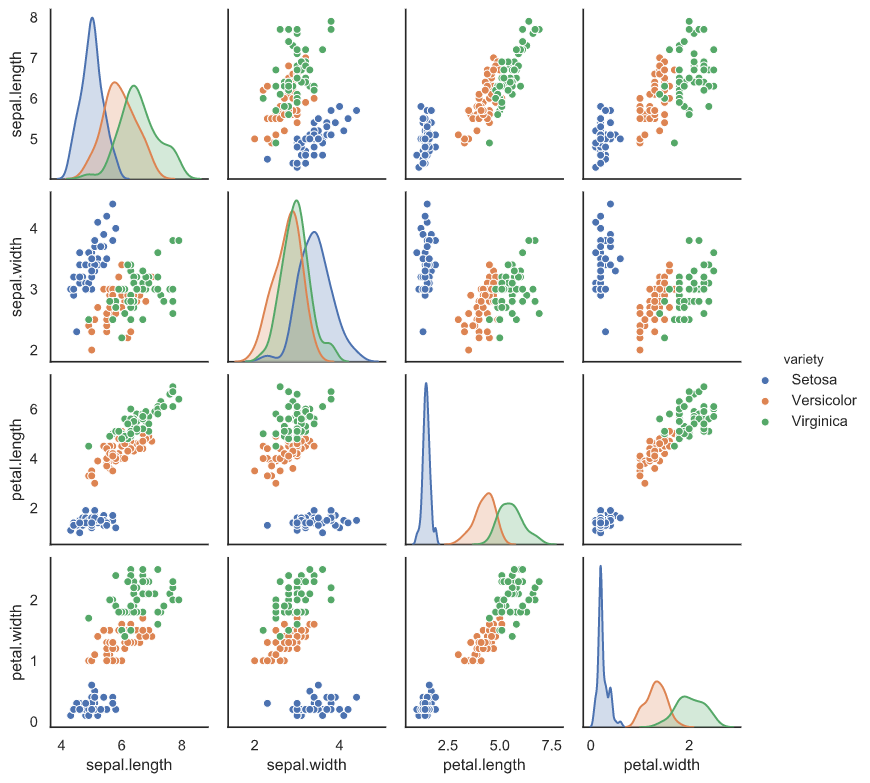
\includegraphics[scale=0.3]{Figures/pair_plot.png}}
\caption{Iris dataset visualization across feature combination.}
\label{fig}
\end{figure}


\subsection{Implementation, result, and discussion}
As mention above, we follow the steps required to perform PCA. We first load the data into our PYTHON environment the above Fig. 1, shows the manipulation of the data. 
The second step of the algorithm consists of standardizing the dataset (zero mean). The following step is to find the eigenvalues and corresponding eigenvectors from the covariance matrix, shown in Fig. 2. and Fig.3. The eigenvectors and eigenvalues of the covariance matrix is the core of PCA: The eigenvectors (principal components) determine the directions of the new feature space, and the eigenvalues determine their magnitude.
In the third step, we choose the top $k$ eigenvectors, the principal component is selected by sorting the eigenvalues in descending order and selecting shown in Fig. 4. The typical goal of a PCA is to reduce the dimensionality of the original feature space by projecting it onto a smaller subspace. To decide which eigenvector(s) can be dropped without losing too much information for the construction of a lower-dimensional subspace, the corresponding eigenvalues must be analyzed. Eigenvectors with the lowest eigenvalues bear the least information about the distribution of the data therefore they can be dropped. The common approach is to rank the eigenvalues from highest to lowest to choose the top $k$ eigenvectors. After deciding which eigenvectors to use, we also choose the number of principal components for the new feature subspace, to do so, we used the explained variance method, obtained from the eigenvalues and that tells us how much variance (extra information) that each component contribute. The plot in Fig. 5, shows that 72.77\% of the variance can be represented by the first principal component. The second principal component carries 23.0\% of information compared to the third and fourth component which can be safely dropped without affecting much the structure of the data. By combining the first two components we obtain 95.8\% of the variance, which means 95.8\% of the information is preserved. 
The last step consists of the projection of the original data onto the new feature space. We use $4\times2$ dimensional eigenvectors to transform our data onto the new subspace, we reduce the dimension from the original 4 dimensions down to 2. Now our new features are represented by $150\times2$ as shown in Fig. 6.
\begin{figure}[h]
\centerline{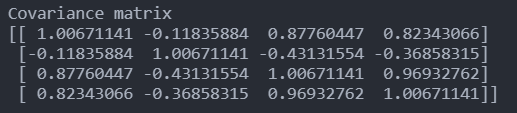
\includegraphics[scale=0.7]{Figures/Covariance Matrix.png}}
\caption{Covariance matrix.}
\label{fig}
\end{figure}

\begin{figure}[h]
\centerline{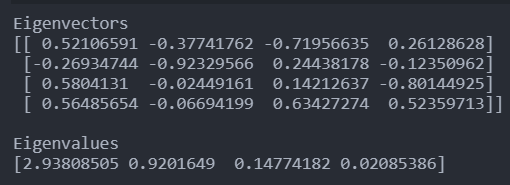
\includegraphics[scale=0.7]{Figures/Eval and Evec.png}}
\caption{Eigenvectors and Eigenvalues.}
\label{fig}
\end{figure}

\begin{figure}[h]
\centerline{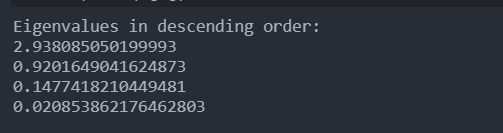
\includegraphics[scale=0.7]{Figures/Ev_sorted.png}}
\caption{Eigenvalues sorted in descending order.}
\label{fig}
\end{figure}

\begin{figure}[h]
\centerline{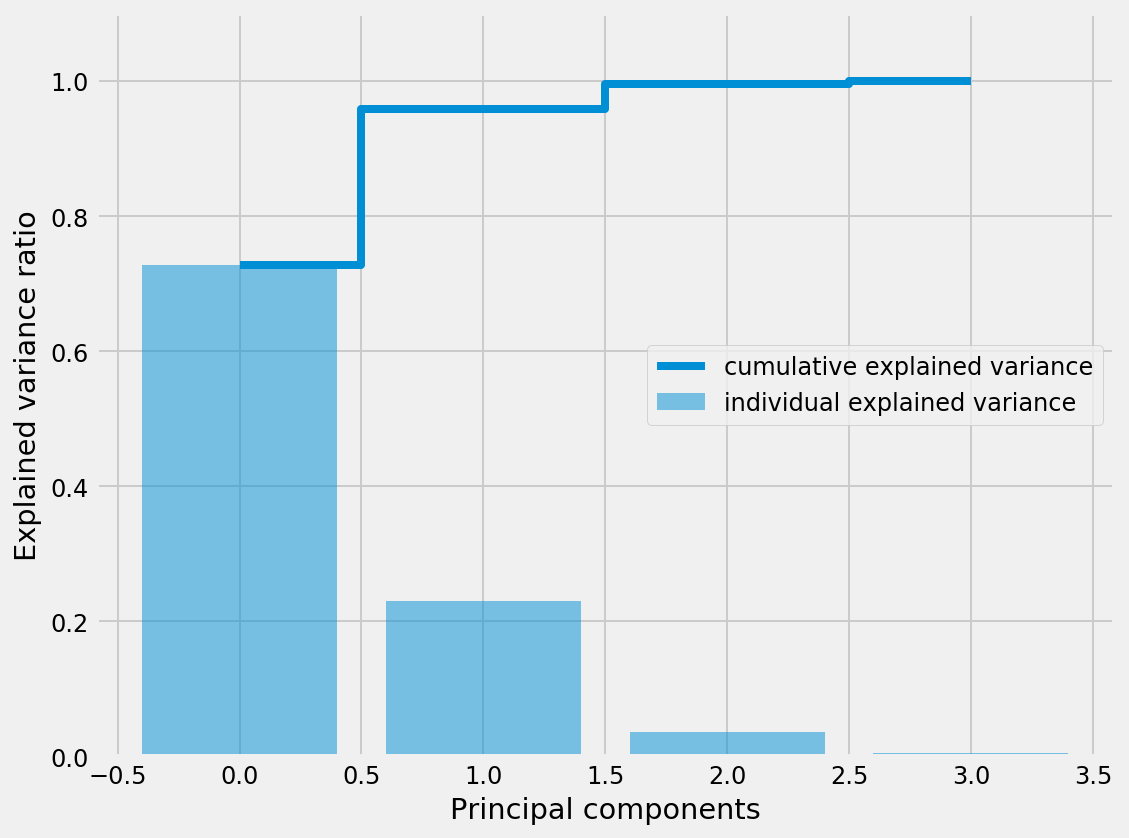
\includegraphics[scale=0.4]{Figures/Variance_exp.png}}
\caption{Cumulative and individual explained variance.}
\label{fig}
\end{figure}

\begin{figure}[h]
\centerline{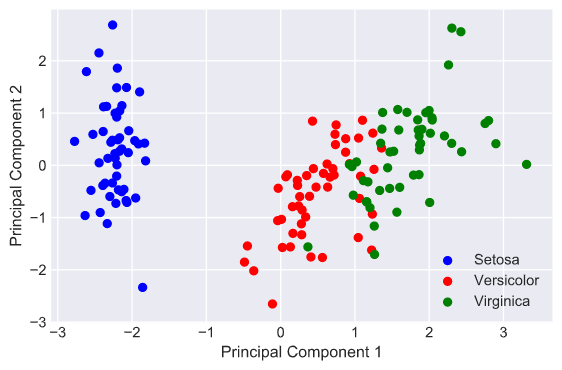
\includegraphics[scale=0.4]{Figures/PC1_PC2_dark.png}}
\caption{Representation of Iris dataset in the new feature space.}
\label{fig}
\end{figure}


\section{Conclusion}

To identify patterns in our data, we often look for disparity across observations to differentiate them from one another. Hence it seems reasonable to be able to find a concise representation that best captures the variation in our initial data. PCA, via its maximum directions of variance, look to explain our data. By compressing a higher dimensional dataset into a lower one, while retaining most of the variance that allows us to perform visualization. Moreover, PCA summarizes our data along with the principal components (or eigenvectors), which explains most of the variance. Therefore, we can reduce the dataset to fewer dimensions and visualize our data's distribution. This can be helpful when we're performing a clustering algorithm that needs to choose the cluster number beforehand. Also, the application of PCA can speed up machine learning algorithms when dealing with Big Data, we might want to reduce the features to a lower dimension, without a significant loss of variance. By performing dimensionality reduction methods, we can reduce the number of features we have to speed up the training algorithm and save memory. 


\begin{thebibliography}{00}
\bibitem{Lamrini} M. Lamrini and M. Y. Chkouri, “Decomposition and Visualization of High-Dimensional Data in a Two Dimensional Interface,” ICSSD 2019 - Int. Conf. Smart Syst. Data Sci., pp. 19–23, 2019, doi: 10.1109/ICSSD47982.2019.9002846.
\bibitem{Genender} A. Genender-Feltheimer, “Visualizing high dimensional and big data,” Procedia Comput. Sci., vol. 140, pp. 112–121, 2018, doi: 10.1016/j.procs.2018.10.308.
\bibitem{Liu} S. Liu, D. Maljovec, B. Wang, P. T. Bremer, and V. Pascucci, “Visualizing High-Dimensional Data: Advances in the Past Decade,” IEEE Trans. Vis. Comput. Graph., vol. 23, no. 3, pp. 1249–1268, 2017, doi: 10.1109/TVCG.2016.2640960.
\bibitem{Onana} F. G. G. and C. A. Onana, “High Dimensional Data Visualization: Advances and Challenges,” Int. J. Comput. Appl., vol. 162, no. March 2017, pp. 23–27, 2017, [Online]. Available: http://www.ijcaonline.org/archives/volume162/number10/27280-2017913362.
\bibitem{Xu} J. Xu, X. Li, and H. Wang, “Extracting Topological Features from Big Data Using Persistent Density Entropy,” J. Phys. Conf. Ser., vol. 1168, no. 3, 2019, doi: 10.1088/1742-6596/1168/3/032017.
\bibitem{Nocke} W. Müller, T. Nocke, and H. Schumann, “Enhancing the visualization process with principal component analysis to support the exploration of trends,” Conf. Res. Pract. Inf. Technol. Ser., vol. 60, no. June 2014, pp. 121–130, 2006, doi: 10.1145/1151903.1151922.
\bibitem{Salem} N. Salem and S. Hussein, “Data dimensional reduction and principal components analysis,” Procedia Comput. Sci., vol. 163, pp. 292–299, 2019, doi: 10.1016/j.procs.2019.12.111.
\bibitem{Houari} R. Houari, A. Bounceur, M. T. Kechadi, A. K. Tari, and R. Euler, “Dimensionality reduction in data mining: A Copula approach,” Expert Syst. Appl., vol. 64, no. October 2017, pp. 247–260, 2016, doi: 10.1016/j.eswa.2016.07.041.
\bibitem{Menon} V. Menon, Q. Du, and J. E. Fowler, “Fast SVD with Random Hadamard Projection for Hyperspectral Dimensionality Reduction,” IEEE Geosci. Remote Sens. Lett., vol. 13, no. 9, pp. 1275–1279, 2016, doi: 10.1109/LGRS.2016.2581172.
\bibitem{Rehman} M. H. ur Rehman, C. S. Liew, A. Abbas, P. P. Jayaraman, T. Y. Wah, and S. U. Khan, “Big Data Reduction Methods: A Survey,” Data Sci. Eng., vol. 1, no. 4, pp. 265–284, 2016, doi: 10.1007/s41019-016-0022-0.
\bibitem{A} A. Tharwat, “Principal component analysis - a tutorial,” Int. J. Appl. Pattern Recognit., vol. 3, no. 3, p. 197, 2016, doi: 10.1504/ijapr.2016.10000630.
\bibitem{D} D. J. Bartholomew, “Principal components analysis,” Int. Encycl. Educ., pp. 374–377, 2010, doi: 10.1016/B978-0-08-044894-7.01358-0.

\end{thebibliography}


\end{document}
